\chapter{Recursive algorithms}

\index{method!value}
\index{method!void}
\index{value method}
\index{void method}

Some of the methods we have used, like the \java{Math} methods, return values.
But all the methods we have {\em written} so far have been \java{void}; that is, they don't return values.
In this chapter, we'll write methods that return values, which we call {\bf value methods}.


\section{Return values}

\index{void}

When you invoke a void method, the invocation is usually on a line all by itself.
For example, here is the \java{countup} method from Section~\ref{recursion}:

\begin{code}
public static void countup(int n) {
    if (n == 0) {
        System.out.println("Blastoff!");
    } else {
        countup(n - 1);
        System.out.println(n);
    }
}
\end{code}

And here is how it is invoked:

\begin{code}
countup(3);
System.out.println("Have a nice day.");
\end{code}

On the other hand, when you invoke a value method, you have to do something with the return value.
We usually assign it to a variable or use it as part of an expression, like this:

\begin{code}
double error = Math.abs(expected - actual);
double height = radius * Math.sin(angle);
\end{code}

\index{value method}
\index{method!value}

Compared to void methods, value methods differ in two ways:

\index{return type}
\index{return value}

\begin{itemize}

\item They declare the type of the return value (the {\bf return type});

\item They use at least one \java{return} statement to provide a {\bf return value}.

\end{itemize}

Here's an example: \java{calculateArea} takes a \java{double} as a parameter and returns the area of a circle with that radius:

\begin{code}
public static double calculateArea(double radius) {
    double result = Math.PI * radius * radius;
    return result;
}
\end{code}

As usual, this method is \java{public} and \java{static}.
But in the place where we are used to seeing \java{void}, we see \java{double}, which means that the return value from this method is a \java{double}.

\index{return}
\index{statement!return}

The last line is a new form of the \java{return} statement that includes a return value.
This statement means, ``return immediately from this method and use the following expression as the return value.''
The expression you provide can be arbitrarily complex, so we could have written this method more concisely:

\begin{code}
public static double calculateArea(double radius) {
    return Math.PI * radius * radius;
}
\end{code}

\index{temporary variable}
\index{variable!temporary}

On the other hand, {\bf temporary variables} like \java{result} often make debugging easier, especially when you are stepping through code using an interactive debugger (see Appendix~\ref{debugger}).

The type of the expression in the \java{return} statement must match the return type of the method.
When you declare that the return type is \java{double}, you are making a promise that this method will eventually produce a \java{double} value.
If you try to \java{return} with no expression, or an expression with the wrong type, the compiler will generate an error.

Sometimes it is useful to have multiple return statements, for example, one in each branch of a conditional:

\begin{code}
public static double absoluteValue(double x) {
    if (x < 0) {
        return -x;
    } else {
        return x;
    }
}
\end{code}

Since these \java{return} statements are in a conditional statement, only one will be executed.
As soon as either of them executes, the method terminates without executing any more statements.

\index{dead code}

Code that appears after a \java{return} statement (in the same block), or any place else where it can never be executed, is called {\bf dead code}.
The compiler will give you an ``unreachable statement'' error if part of your code is dead.
For example, this method contains dead code:

\begin{code}
public static double absoluteValue(double x) {
    if (x < 0) {
        return -x;
    } else {
        return x;
    }
    System.out.println("This line is dead.");
}
\end{code}

If you put \java{return} statements inside a conditional statement, you have to make sure that {\em every possible path} through the program reaches a \java{return} statement.
The compiler will let you know if that's not the case.
For example, the following method is incomplete:

\begin{code}
public static double absoluteValue(double x) {
    if (x < 0) {
        return -x;
    } else if (x > 0) {
        return x;
    }
    // syntax error
}
\end{code}

When \java{x} is 0, neither condition is true, so the method ends without hitting a return statement.
The error message in this case might be something like ``missing return statement'', which is confusing since there are already two of them.
But hopefully you will know what it means.


\section{Writing methods}
\label{distance}

\index{incremental development}
\index{program development}

Beginners often make the mistake of writing a lot of code before they try to compile and run it.
Then they spend way too much time debugging.
A better approach is what we call {\bf incremental development}.
The key aspects of incremental development are:

\begin{itemize}

\item Start with a working program and make small, incremental changes.
At any point, if there is an error, you will know where to look.

\item Use variables to hold intermediate values so you can check them, either with print statements or by using a debugger.

\item Once the program is working, you can consolidate multiple statements into compound expressions (but only if it does not make the program more difficult to read).

\end{itemize}

As an example, suppose you want to find the distance between two points, given by the coordinates $(x_1, y_1)$ and $(x_2, y_2)$.
By the usual definition:

\[ distance = \sqrt{(x_2 - x_1)^2 +(y_2 - y_1)^2} \]

The first step is to consider what a \java{distance} method should look like in Java.
In other words, what are the inputs (parameters) and what is the output (return value)?
In this case, the two points are the parameters, and it is natural to represent them using four \java{double} values.
%, although we will see later that there is a \java{Point} object in Java that we could use.
The return value is the distance, which should also have type \java{double}.

\index{stub}

Already we can write an outline for the method, which is sometimes called a {\bf stub}.
The stub includes the method signature and a \java{return} statement:

\begin{code}
public static double distance
        (double x1, double y1, double x2, double y2) {
    return 0.0;
}
\end{code}

The return statement is a placeholder that is necessary for the program to compile.
At this stage the program doesn't do anything useful, but it is good to compile it so we can find any syntax errors before we add more code.

It's usually a good idea to think about testing {\em before} you develop new methods; doing so can help you figure out how to implement them.
To test the method, we can invoke it from \java{main} using sample values:

\begin{code}
double dist = distance(1.0, 2.0, 4.0, 6.0);
\end{code}

With these values, the horizontal distance is 3.0 and the vertical distance is 4.0.
So the result should be 5.0, the hypotenuse of a 3-4-5 triangle.
When you are testing a method, it is helpful to know the right answer.

Once we have compiled the stub, we can start adding lines of code one at a time.
After each incremental change, we recompile and run the program.
If there is an error at any point, we have a good idea where to look: the last line we added.

The next step is to find the differences $x_2 - x_1$ and $y_2 - y_1$.
We store those values in temporary variables named \java{dx} and \java{dy}.

\begin{code}
public static double distance
        (double x1, double y1, double x2, double y2) {
    double dx = x2 - x1;
    double dy = y2 - y1;
    System.out.println("dx is " + dx);
    System.out.println("dy is " + dy);
    return 0.0;
}
\end{code}

\index{scaffolding}

The print statements allows us to check the intermediate values before proceeding.
They should be 3.0 and 4.0.
We will remove the print statements when the method is finished.
Code like that is called {\bf scaffolding}, because it is helpful for building the program, but it is not part of the final product.

The next step is to square \java{dx} and \java{dy}.
We could use the \java{Math.pow} method, but it is simpler to multiply each term by itself.

\begin{code}
public static double distance
        (double x1, double y1, double x2, double y2) {
    double dx = x2 - x1;
    double dy = y2 - y1;
    double dsquared = dx * dx + dy * dy;
    System.out.println("dsquared is " + dsquared);
    return 0.0;
}
\end{code}

Again, you should compile and run the program at this stage and check the intermediate value, which should be 25.0.
Finally, we can use \java{Math.sqrt} to compute and return the result.

\begin{code}
public static double distance
        (double x1, double y1, double x2, double y2) {
    double dx = x2 - x1;
    double dy = y2 - y1;
    double dsquared = dx * dx + dy * dy;
    double result = Math.sqrt(dsquared);
    return result;
}
\end{code}

%In \java{main}, we can print and check the value of the result.

As you gain more experience programming, you might write and debug more than one line at a time.
Nevertheless, incremental development can save you a lot of time.


\section{Method composition}

\index{composition}

Once you define a new method, you can use it as part of an expression, or build new methods using existing methods.
For example, suppose someone gave you two points, the center of the circle and a point on the perimeter, and asked for the area of the circle.
Let's say the center point is stored in the variables \java{xc} and \java{yc}, and the perimeter point is in \java{xp} and \java{yp}.

The first step is to find the radius of the circle, which is the distance between the two points.
Fortunately, we have a method that does just that (\java{distance}).

\begin{code}
double radius = distance(xc, yc, xp, yp);
\end{code}

The second step is to find the area of a circle with that radius.
We have a method for that computation too (\java{calculateArea}).

\begin{code}
double area = calculateArea(radius);
return area;
\end{code}

Putting everything together in a new method, we get:

\begin{code}
public static double circleArea
        (double xc, double yc, double xp, double yp) {
    double radius = distance(xc, yc, xp, yp);
    double area = calculateArea(radius);
    return area;
}
\end{code}

The temporary variables \java{radius} and \java{area} are useful for development and debugging, but once the program is working we can make it more concise by composing the method calls:

\begin{code}
public static double circleArea
        (double xc, double yc, double xp, double yp) {
    return calculateArea(distance(xc, yc, xp, yp));
}
\end{code}

\index{functional decomposition}

This example demonstrates a process called {\bf functional decomposition}; that is, breaking a complex computation into simple methods, testing the methods in isolation, and then composing the methods to perform the computation.
This process reduces debugging time and yields code that is more likely to be correct and easier to maintain.

%Computer scientists deal with the complexity of large programs by breaking down computations into simple methods (which in turn may call other methods).
%Data is passed around the program via method parameters and return statements.
%By using incremental development, scaffolding, and testing, you can be confident that your code is correct.


\section{Overloading}
\label{overloading}

You might have noticed that \java{circleArea} and \java{calculateArea} perform similar functions.
They both find the area of a circle, but they take different parameters.
For \java{calculateArea}, we have to provide the radius; for \java{circleArea} we provide two points.

\index{overload}

If two methods do the same thing, it is natural to give them the same name.
Having more than one method with the same name is called {\bf overloading}, and it is legal in Java as long as each version takes different parameters.
So we could rename \java{circleArea} to \java{calculateArea}:

\begin{code}
public static double calculateArea
        (double xc, double yc, double xp, double yp) {
    return calculateArea(distance(xc, yc, xp, yp));
}
\end{code}

Note that this new \java{calculateArea} method is {\em not} recursive.
When you invoke an overloaded method, Java knows which version you want by looking at the arguments that you provide.
If you write:

\begin{code}
double x = calculateArea(3.0);
\end{code}

Java looks for a method named \java{calculateArea} that takes one \java{double} as an argument, and so it uses the first version, which interprets the argument as a radius.
If you write:

\begin{code}
double y = calculateArea(1.0, 2.0, 4.0, 6.0);
\end{code}

Java uses the second version of \java{calculateArea}, which interprets the arguments as two points.
In this example, the second version actually invokes the first version.

Many Java methods are overloaded, meaning that there are different versions that accept different numbers or types of parameters.
For example, there are versions of \java{print} and \java{println} that accept a single parameter of any data type.
In the \java{Math} class, there is a version of \java{abs} that works on \java{double}s, and there is also a version for \java{int}s.

Although overloading is a useful feature, it should be used with caution.
You might get yourself nicely confused if you are trying to debug one version of a method while accidentally invoking a different one.


\section{Boolean methods}
\label{boolean}

\index{boolean}
\index{method!boolean}

Methods can return \java{boolean} values, just like any other type, which is often convenient for hiding tests inside methods.
For example:

\begin{code}
public static boolean isSingleDigit(int x) {
    if (x > -10 && x < 10) {
        return true;
    } else {
        return false;
    }
}
\end{code}

The name of this method is \java{isSingleDigit}.
It is common to give \java{boolean} methods names that sound like yes/no questions.
Since the return type is \java{boolean}, the return statement has to provide a boolean expression.

The code itself is straightforward, although it is longer than it needs to be.
Remember that the expression \java{x > -10 && x < 10} has type \java{boolean}, so there is nothing wrong with returning it directly (without the \java{if} statement):

\begin{code}
public static boolean isSingleDigit(int x) {
    return x > -10 && x < 10;
}
\end{code}

In \java{main}, you can invoke the method in the usual ways:

\begin{code}
System.out.println(isSingleDigit(2));
boolean bigFlag = !isSingleDigit(17);
\end{code}

The first line displays \java{true} because 2 is a single-digit number.
The second line sets \java{bigFlag} to \java{true}, because 17 is {\em not} a single-digit number.

Conditional statements often invoke \java{boolean} methods and use the result as the condition:

\begin{code}
if (isSingleDigit(z)) {
    System.out.println("z is small");
} else {
    System.out.println("z is big");
}
\end{code}

Examples like this one almost read like English:
``If is single digit z, print ... else print ...''.


\section{Javadoc tags}

In Section~\ref{sec:javadoc}, we discussed how to write documentation comments using \java{/**}.
It's generally a good idea to document each class and method, so that other programmers can understand what they do without having to read the code.

\index{tag}
\index{param tag}
\index{return tag}
\index{documentation!Javadoc tags}

To organize the documentation into sections, Javadoc supports optional {\bf tags} that begin with the at sign (\java{@}).
For example, we can use \java{@param} and \java{@return} to provide additional information about parameters and return values.

\begin{code}
/**
 * Tests whether x is a single digit integer.
 *
 * @param x the integer to test
 * @return true if x has one digit, false otherwise
 */
public static boolean isSingleDigit(int x) {
\end{code}

\index{HTML}
\index{Javadoc}

Figure~\ref{fig.javadoc} shows part of the resulting HTML page generated by Javadoc.
Notice the relationship between the source code and the documentation.

\begin{figure}[!ht]
\begin{center}
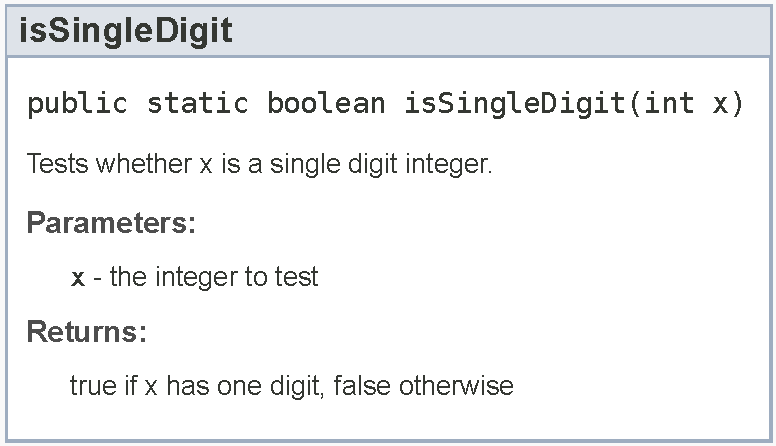
\includegraphics[scale=0.8]{figs/javadoc.pdf}
\caption{HTML documentation for \java{isSingleDigit}.}
\label{fig.javadoc}
\end{center}
\end{figure}

Methods with multiple parameters should have separate \java{@param} tags that describe each one.
Void methods should have no \java{@return} tag, since they do not return a value.


\section{More recursion}
\label{factorial}

\index{Turing complete}
\index{language!complete}

\index{Turing, Alan}
\index{Church, Alonzo}

Now that we have methods that return values, we have a {\bf Turing complete} programming language.
That means Java can compute anything computable, for any reasonable definition of ``computable''.
This idea was developed by Alonzo Church and Alan Turing, so it is known as the Church-Turing thesis.
%You can read more about it at \url{https://en.wikipedia.org/wiki/Turing_thesis}.

\index{recursion}

To give you an idea of what you can do with the tools we have learned, let's look at some methods for evaluating recursively-defined mathematical functions.
A recursive definition is similar to a circular definition, in the sense that the definition refers to the thing being defined.

Of course, a truly circular definition is not very useful:

\begin{description}
\term{recursive} An adjective used to describe a method that is recursive.
\end{description}

If you saw that definition in the dictionary, you might be annoyed.
But if you search for recursion on Google, it displays ``Did you mean: recursion'' as an inside joke.

\index{factorial}

Many mathematical functions are defined recursively, because that is often the simplest way.
For example, the {\bf factorial} of an integer $n$, which is written $n!$, is defined like this:
%
\begin{eqnarray*}
&&  0! = 1 \\
&&  n! = n \cdot(n-1)!
\end{eqnarray*}

Don't confuse the mathematical symbol $!$, which means {\em factorial}, with the Java operator \java{!}, which means {\em not}.
This definition says that \java{factorial(0)} is \java{1}, and that \java{factorial(n)} is \java{n * factorial(n - 1)}.

So \java{factorial(3)} is \java{3 * factorial(2)}; \java{factorial(2)} is \java{2 * factorial(1)}; \java{factorial(1)} is \java{1 * factorial(0)}; and \java{factorial(0)} is \java{1}.
Putting it all together, we get \java{3 * 2 * 1 * 1}, which is 6.

If you can formulate a recursive definition of something, you can easily write a Java method to evaluate it.
The first step is to decide what the parameters and return type are.
Since factorial is defined for integers, the method takes an \java{int} as a parameter and returns an \java{int}.
So here's a good starting place:

\begin{code}
public static int factorial(int n) {
    return 0;
}
\end{code}

Next, we think about the base case.
If the argument happens to be zero, we return 1.

\begin{code}
public static int factorial(int n) {
    if (n == 0) {
        return 1;
    }
    return 0;
}
\end{code}

Otherwise, and this is the interesting part, we have to make a recursive call to find the factorial of $n-1$, and then multiply it by $n$.

\begin{code}
public static int factorial(int n) {
    if (n == 0) {
        return 1;
    }
    int recurse = factorial(n - 1);
    int result = n * recurse;
    return result;
}
\end{code}

The flow of execution for this program is similar to \java{countdown} from Section~\ref{recursion}.
If we invoke \java{factorial} with the value 3:

\vspace{-1ex}
\begin{quote}
Since 3 is not zero, we take the second branch and calculate the factorial of $n-1$...
\begin{quote}
Since 2 is not zero, we take the second branch and calculate the factorial of $n-1$...
\begin{quote}
Since 1 is not zero, we take the second branch and calculate the factorial of $n-1$...
\begin{quote}
Since 0 {\em is} zero, we take the first branch and return the value 1 immediately.
% without making any more recursive invocations.
\end{quote}
The return value (1) gets multiplied by \java{n}, which is 1, and the result is returned.
\end{quote}
The return value (1) gets multiplied by \java{n}, which is 2, and the result is returned.
\end{quote}
The return value (2) gets multiplied by \java{n}, which is 3, and the result, 6, is returned to whatever invoked \java{factorial(3)}.
\end{quote}
\vspace{-1ex}

\index{stack}
\index{diagram!stack}

Figure~\ref{fig.stack3} shows what the stack diagram looks like for this sequence of method invocations.
The return values are shown being passed back up the stack.
Notice that \java{recurse} and \java{result} do not exist in the last frame, because when \java{n == 0} the code that declares them does not execute.

\begin{figure}[!ht]
\begin{center}
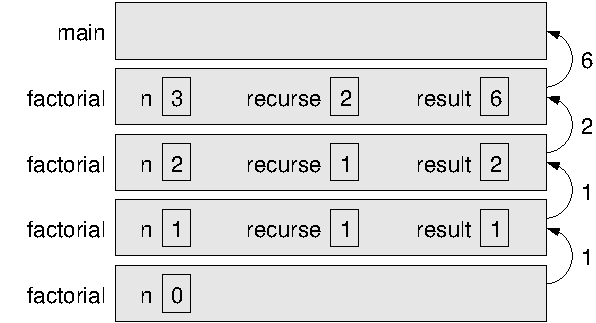
\includegraphics{figs/stack3.pdf}
\caption{Stack diagram for the \java{factorial} method.}
\label{fig.stack3}
\end{center}
\end{figure}


\section{Leap of faith}
\label{leap of faith}

\index{leap of faith}

Following the flow of execution is one way to read programs, but it can quickly become overwhelming.
An alternative is the {\bf leap of faith}:
when you come to a method invocation, instead of following the flow of execution, you {\em assume} that the method works correctly and returns the appropriate value.

In fact, you are already practicing a leap of faith when you use methods in the Java library.
When you invoke \java{Math.cos} or \java{System.out.println}, you don't examine the implementations of those methods.
You just assume that they work properly.

You should apply the same reasoning to your own methods.
For example, in Section~\ref{boolean} we wrote a method called \java{isSingleDigit} that determines whether a number is between 0 and 9.
Once we convince ourselves that this method is correct -- by testing and examination of the code -- we can use the method without ever looking at the implementation again.

The same is true of recursive methods.
When you get to the recursive call, instead of following the flow of execution you should {\em assume} that the recursive invocation works.
For example, ``Assuming that I can find the factorial of $n-1$, can I compute the factorial of $n$?''
Yes you can, by multiplying by $n$.

Of course, it is strange to assume that the method works correctly when you have not finished writing it, but that's why it's called a leap of faith!


\section{One more example}
\label{fibonacci}

\index{fibonacci}

Another common recursively-defined mathematical function is the Fibonacci sequence, which has the following definition:
%
\begin{eqnarray*}
&& fibonacci(1) = 1 \\
&& fibonacci(2) = 1 \\
&& fibonacci(n) = fibonacci(n-1) + fibonacci(n-2)
\end{eqnarray*}

Translated into Java, this function is:

\begin{code}
public static int fibonacci(int n) {
    if (n == 1 || n == 2) {
        return 1;
    }
    return fibonacci(n - 1) + fibonacci(n - 2);
}
\end{code}

If you try to follow the flow of execution here, even for small values of \java{n}, your head will explode.
But if we take a leap of faith and assume that the two recursive invocations work correctly, it is clear that their sum is the result.


\section{Vocabulary}

\begin{description}

\term{void method}
A method that does not return a value.

\term{value method}
A method that returns a value.

%\term{void}
%A special return type indicating the method does not return a value.

\term{return type}
The type of value a method returns.

\term{return value}
The value provided as the result of a method invocation.

\term{temporary variable}
A short-lived variable, often used for debugging.

\term{dead code}
Part of a program that can never be executed, often because it appears after a \java{return} statement.

\term{incremental development}
A process for creating programs by writing a few lines at a time, compiling, and testing.

\term{stub}
A placeholder for an incomplete method so that the class will compile.

\term{scaffolding}
Code that is used during program development but is not part of the final version.

\term{functional decomposition}
A process for breaking down a complex computation into simple methods, then composing the methods to perform the computation.

\term{overload}
To define more than one method with the same name but different parameters.
%When you invoke an overloaded method, Java knows which version to use by looking at the arguments you provide.

\term{tag}
A label that begins with an at sign (\java{@}) and is used by Javadoc to organize documentation into sections.

\term{Turing complete}
A programming language that can implement any theoretically possible algorithm.

\term{factorial}
The product of all the integers up to and including a given integer.

\term{leap of faith}
A way to read recursive programs by assuming that the recursive call works, rather than following the flow of execution.

\end{description}


\section{Exercises}

The code for this chapter is in the {\tt ch08} directory of {\tt ThinkJava2Code}.
See page~\pageref{code} for instructions on how to download the repository.
Before you start the exercises, we recommend that you compile and run the examples.

If you have not already read Appendix~\ref{JUnit}, now might be a good time.
It describes JUnit, a tool for efficiently testing value methods.


\begin{exercise}

If you have a question about whether something is legal, and what happens if it is not, a good way to find out is to ask the compiler.
Answer the following questions by trying them out.

\begin{enumerate}

\item What happens if you invoke a value method and don't do anything with the result; that is, if you don't assign it to a variable or use it as part of a larger expression?

\item What happens if you use a void method as part of an expression?
For example, try \java{System.out.println("boo!") + 7;}

\end{enumerate}

\end{exercise}


\begin{exercise}
\label{ex.isdiv}

Write a method named \java{isDivisible} that takes two integers, \java{n} and \java{m}, and that returns \java{true} if \java{n} is divisible by \java{m}, and \java{false} otherwise.

\end{exercise}


\begin{exercise}

If you are given three sticks, you may or may not be able to arrange them in a triangle.
For example, if one of the sticks is 12 inches long and the other two are one inch long, you will not be able to get the short sticks to meet in the middle.
For any three lengths, there is a simple test to see if it is possible to form a triangle:

\begin{quotation}
\noindent
If any of the three lengths is greater than the sum of the other two, you cannot form a triangle.
\end{quotation}

Write a method named \java{isTriangle} that takes three integers as arguments and returns either \java{true} or \java{false}, depending on whether you can or cannot form a triangle from sticks with the given lengths.
The point of this exercise is to use conditional statements to write a value method.

\end{exercise}


\begin{exercise}
\label{ex.multadd}

Many computations can be expressed more concisely using the ``multadd'' operation, which takes three operands and computes \java{a * b + c}.
Some processors even provide a hardware implementation of this operation for floating-point numbers.

\begin{enumerate}

\item Create a new program called {\tt Multadd.java}.

\item Write a method called \java{multadd} that takes three \java{doubles} as parameters and that returns \java{a * b + c}.

\item Write a \java{main} method that tests \java{multadd} by invoking it with a few simple parameters, like \java{1.0, 2.0, 3.0}.

\item Also in \java{main}, use \java{multadd} to compute the following values:
%
\begin{eqnarray*}
& \sin \frac{\pi}{4} + \frac{\cos \frac{\pi}{4}}{2} & \\
& \log 10 + \log 20 &
\end{eqnarray*}

\item Write a method called \java{expSum} that takes a double as a parameter and that uses \java{multadd} to calculate:
%
\begin{eqnarray*}
x e^{-x} + \sqrt{1 - e^{-x}}
\end{eqnarray*}
%
{\it Hint:} The method for raising $e$ to a power is \java{Math.exp}.

\end{enumerate}

In the last part of this exercise, you need to write a method that invokes another method you wrote.
Whenever you do that, it is a good idea to test the first method carefully before working on the second.
Otherwise, you might find yourself debugging two methods at the same time, which can be difficult.

One of the purposes of this exercise is to practice pattern-matching: the ability to recognize a specific problem as an instance of a general category of problems.

\end{exercise}


\begin{exercise}

What is the output of the following program?

\begin{code}
public static void main(String[] args) {
    boolean flag1 = isHoopy(202);
    boolean flag2 = isFrabjuous(202);
    System.out.println(flag1);
    System.out.println(flag2);
    if (flag1 && flag2) {
        System.out.println("ping!");
    }
    if (flag1 || flag2) {
        System.out.println("pong!");
    }
}
\end{code}

\begin{code}
public static boolean isHoopy(int x) {
    boolean hoopyFlag;
    if (x % 2 == 0) {
        hoopyFlag = true;
    } else {
        hoopyFlag = false;
    }
    return hoopyFlag;
}
\end{code}

\begin{code}
public static boolean isFrabjuous(int x) {
    boolean frabjuousFlag;
    if (x > 0) {
        frabjuousFlag = true;
    } else {
        frabjuousFlag = false;
    }
    return frabjuousFlag;
}
\end{code}

The purpose of this exercise is to make sure you understand logical operators and the flow of execution through value methods.

\end{exercise}


\begin{exercise}

In this exercise, you will use a stack diagram to understand the execution of the following recursive program.

\begin{code}
public static void main(String[] args) {
    System.out.println(prod(1, 4));
}

public static int prod(int m, int n) {
    if (m == n) {
        return n;
    } else {
        int recurse = prod(m, n - 1);
        int result = n * recurse;
        return result;
    }
}
\end{code}

\begin{enumerate}

\item Draw a stack diagram showing the state of the program just before the last invocation of \java{prod} completes.

\item What is the output of this program?
(Try to answer this question on paper first, then run the code to check your answer.)

\item Explain in a few words what \java{prod} does (without getting into the details of how it works).

\item Rewrite \java{prod} without the temporary variables \java{recurse} and \java{result}.
{\it Hint:} You only need one line for the \java{else} branch.

\end{enumerate}

\end{exercise}


\begin{exercise}
Write a recursive method named \java{oddSum} that takes a positive odd integer \java{n} and returns the sum of odd integers from 1 to n.
Start with a base case, and use temporary variables to debug your solution.
You might find it helpful to print the value of \java{n} each time \java{oddSum} is invoked.
\end{exercise}


\begin{exercise}

The goal of this exercise is to translate a recursive definition into a Java method.
The Ackermann function is defined for non-negative integers as follows:
\begin{eqnarray*}
A(m, n) = \begin{cases}
              n+1 & \mbox{if } m = 0 \\
        A(m-1, 1) & \mbox{if } m > 0 \mbox{ and } n = 0 \\
A(m-1, A(m, n-1)) & \mbox{if } m > 0 \mbox{ and } n > 0
\end{cases}
\end{eqnarray*}

Write a method called \java{ack} that takes two \java{int}s as parameters and that computes and returns the value of the Ackermann function.

Test your implementation of Ackermann by invoking it from \java{main} and displaying the return value.
Note the return value gets very big very quickly.
You should try it only for small values of $m$ and $n$ (not bigger than 3).

\end{exercise}


\begin{exercise}
\label{ex.power}

Write a recursive method called \java{power} that takes a double \java{x} and an integer \java{n} and returns $x^n$.

{\it Hint:} A recursive definition of this operation is $x^n = x \cdot x^{n-1}$.
Also, remember that anything raised to the zeroth power is 1.

Optional challenge: you can make this method more efficient, when \java{n} is even, using $x^n = \left( x^{n/2} \right)^2$.

\end{exercise}
